% !TeX program = lualatex
% !TeX encoding = utf8
% !TeX spellcheck = uk_UA
% !BIB program = biber
% !TeX root =../QChemBook.tex
\graphicspath{ {\currfiledir/Pictures/} }

\chapter{Рівняння Хартрі-Фока}

Навіть з урахуванням наближення Борна-Оппенгеймера, яке дозволило розділити атомно-молекулярну систему на дві підсистеми~--- ядерну і електронну,~--- нам все ще не вдається розв'язати рівняння Шредінґера, яке для електронної підсистеми має вигляд:

\begin{equation}\label{eq:Shredinger_eq_el_subsystem}
	\left( -\frac12 \sum\limits_{i = 1}^N  \nabla^2_i
    + \frac12 \sum\limits_{\alpha \neq \beta}^K \frac{Z_\alpha Z_\beta}{R_{\alpha\beta}}
    - \sum\limits_{\alpha = 1}^K  \sum\limits_{i = 1}^N \frac{Z_\alpha}{R_{\alpha i}}
    + \frac12 \sum\limits_{i = 1}^N \sum\limits_{j \neq j}^N \frac{1}{r_{ij}} \right)  \Phi (\vect{r}, \sigma | \vect{R}) = E_\mathrm{el} \Phi (\vect{r}, \sigma | \vect{R}) .
\end{equation}

Основною причиною цього є останній доданок $\frac12 \sum\limits_{i = 1}^N \sum\limits_{j \neq j}^N \frac{1}{r_{ij}}$, що описує електрон-електронну взаємодію. Саме його наявність не дозволяє розділити змінні в рівнянні. Крім того, фізично, така неможливість відокремити змінні говорить про те, що не можна визначити стани окремих електронів в системі. Спроба врахувати цей доданок за допомогою теорії збурень призводить до поганих результатів, оскільки взаємодія між електронами має той же порядок, що і взаємодія електронів з ядром. 


\section{Одноелектронне наближення}

\begin{wrapfigure}[14]{O}[0pt]{5cm}
\begin{center}
	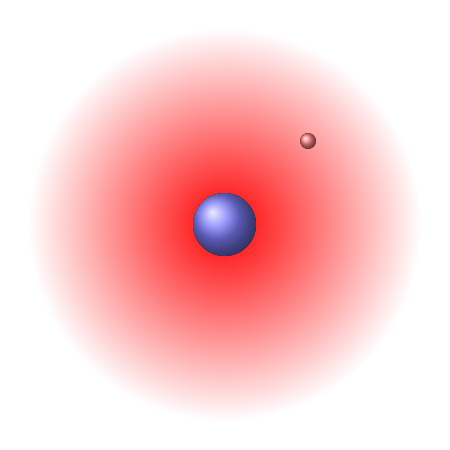
\begin{tikzpicture}
 		\path[inner color=red, outer color=white] (0,0) circle(2.5);
		\fill[ball color=blue!50] (0,0) circle (0.4);
		\fill[ball color=red!50]  (45:1.5) coordinate (E2) circle (0.1);
	\end{tikzpicture}
	\captionof{figure}{Ілюстрація методу одноелектронного наближення.}
	\label{pic:SCF_explanation}
\end{center}
\end{wrapfigure}
Основним наближенням, яке використовується в квантовій хімії є \emph{одноелектронне} наближення. В його основі лежить уявлення про існування індивідуальних станів кожного електрона, які являють собою стаціонарні стани руху електрона в деякому ефективному центральносиметричному полі, яке створюється ядром (або ядрами) і всіма іншими електронами (рис.~\ref{pic:SCF_explanation}). Іншими словами, у рамках такого наближення кожен електрон багатоелектронної системи є немов би незалежним. Для реалізації такого наближення останній доданок в гамільтоніані~\eqref{HeliumAthomHamiltonian} можна замінити на наближений:
\begin{equation}
	\frac12 \sum\limits_{i}^{N}\sum\limits_{\substack{j,\, j \neq i}}^{N}\frac{1}{r_{ij}} \approx \sum\limits_{i}^{N} \overline{V}(r_i),
\end{equation}
де потенціал $\overline{V}(r)$ може бути витлумачений як потенціал взаємодії електрона з розподіленим за об'ємом атома зарядом інших електронів. Важливо підкреслити, що взаємодія електрона залежить не від одночасного положення всіх інших електронів, а саме від їх усередненого положення. Потенціал $\overline{V}(r)$ також називають самоузгодженим, оскільки він залежить від стану атома, яке в свою чергу залежить від $\overline{V}(r)$. Тоді гамільтоніан системи можна представити у вигляді суми одночастинових гамільтоніанів, а отже, дає можливість розділити змінні. Цей гамільтоніан має вигляд:
\begin{equation}\label{approx_Hamiltonian}
	\hat{H}' = \sum\limits_{i}^{N}\hat{h}_i = -\frac12 \sum\limits_{i}^{N} \vect{\nabla}^2_i + \sum\limits_{i}^{N} \left( -\frac{Z}{r_i} + \overline{V}(r_i)\right).
\end{equation}


Таким чином, гамільтоніан \eqref{ManyAthomHamiltonian} $\hat{H}$ апроксимується гамільтоніаном \eqref {approx_Hamiltonian} $\hat{H}'$, а різницю $\hat{H}' - \hat{H} = W$ можна вважати збуренням і врахувати методом теорії збурень.